\chapter{Fundamentals of Retrieval-Augmented Generation}
\label{chap:fundamentals_rag}

Retrieval-Augmented Generation (RAG) is an architectural pattern for LLM-based systems that combines a retrieval component with a generative model. This approach enhances the model's knowledge with external, up-to-date information, addressing common limitations like knowledge cutoffs and hallucination \autocite{lewis2020retrieval, gao2024retrievalaugmented}. This chapter establishes the foundational understanding by elucidating the core mechanics of RAG, its principal challenges, and the function of its key components.

\section{How it Works}
The foundational RAG architecture, frequently termed \textbf{Naive RAG} \autocite{gao2024retrievalaugmented}, functions through two primary stages: retrieval and generation, as initially posited by Lewis et al. (2020) \autocite{lewis2020retrieval}. This paradigm was significantly influenced by earlier and parallel developments in dense retrieval and knowledge-augmented language models, such as Dense Passage Retrieval (DPR) by Karpukhin et al. (2020) \autocite{karpukhin2020dense} and REALM (Retrieval-Augmented Language Model) by Guu et al. (2020) \autocite{guu2020realm}, which laid crucial groundwork for effectively integrating external knowledge. The process commences upon a user's query submission. Rather than directly inputting the query to the LLM, the RAG pipeline first intercepts and processes it by interacting with an external knowledge base.

\begin{enumerate}
    \item \textbf{Retrieval Stage:} The primary objective of this stage is to efficiently identify and extract the most pertinent information from an extensive external knowledge base to facilitate the answering of the user's query. The user's query is transformed into a vector representation, termed the \textit{embedding}, utilizing a text embedding model. This query embedding is then used to search a pre-indexed collection of documents. The objective is to identify and retrieve text segments that exhibit semantic similarity to the query. This retrieval is typically executed utilizing a vector database, which is engineered for high-throughput similarity searches across extensive datasets of embeddings. The output of this stage comprises a set of pertinent text segments, frequently designated as the \textit{context}.

    
    \item \textbf{Generation Stage:} In this stage, the Large Language Model (LLM) functions as a sophisticated text synthesizer. The objective of this stage is to generate a coherent and factually accurate response by leveraging the retrieved information, a process frequently termed knowledge-grounded generation \autocite{yu2022survey}. The retrieved context is then combined with the original query into a structured prompt. This augmented prompt is fed to the LLM. By providing this explicit, pertinent information, the LLM is directed to produce a response that is not only contextually appropriate but also substantiated by the facts contained within the retrieved documents, thereby minimizing reliance on its internal, potentially outdated or erroneous, knowledge. This process substantially enhances the accuracy and factuality of the output.
\end{enumerate}

\begin{figure}[!htbp]
    \centering
    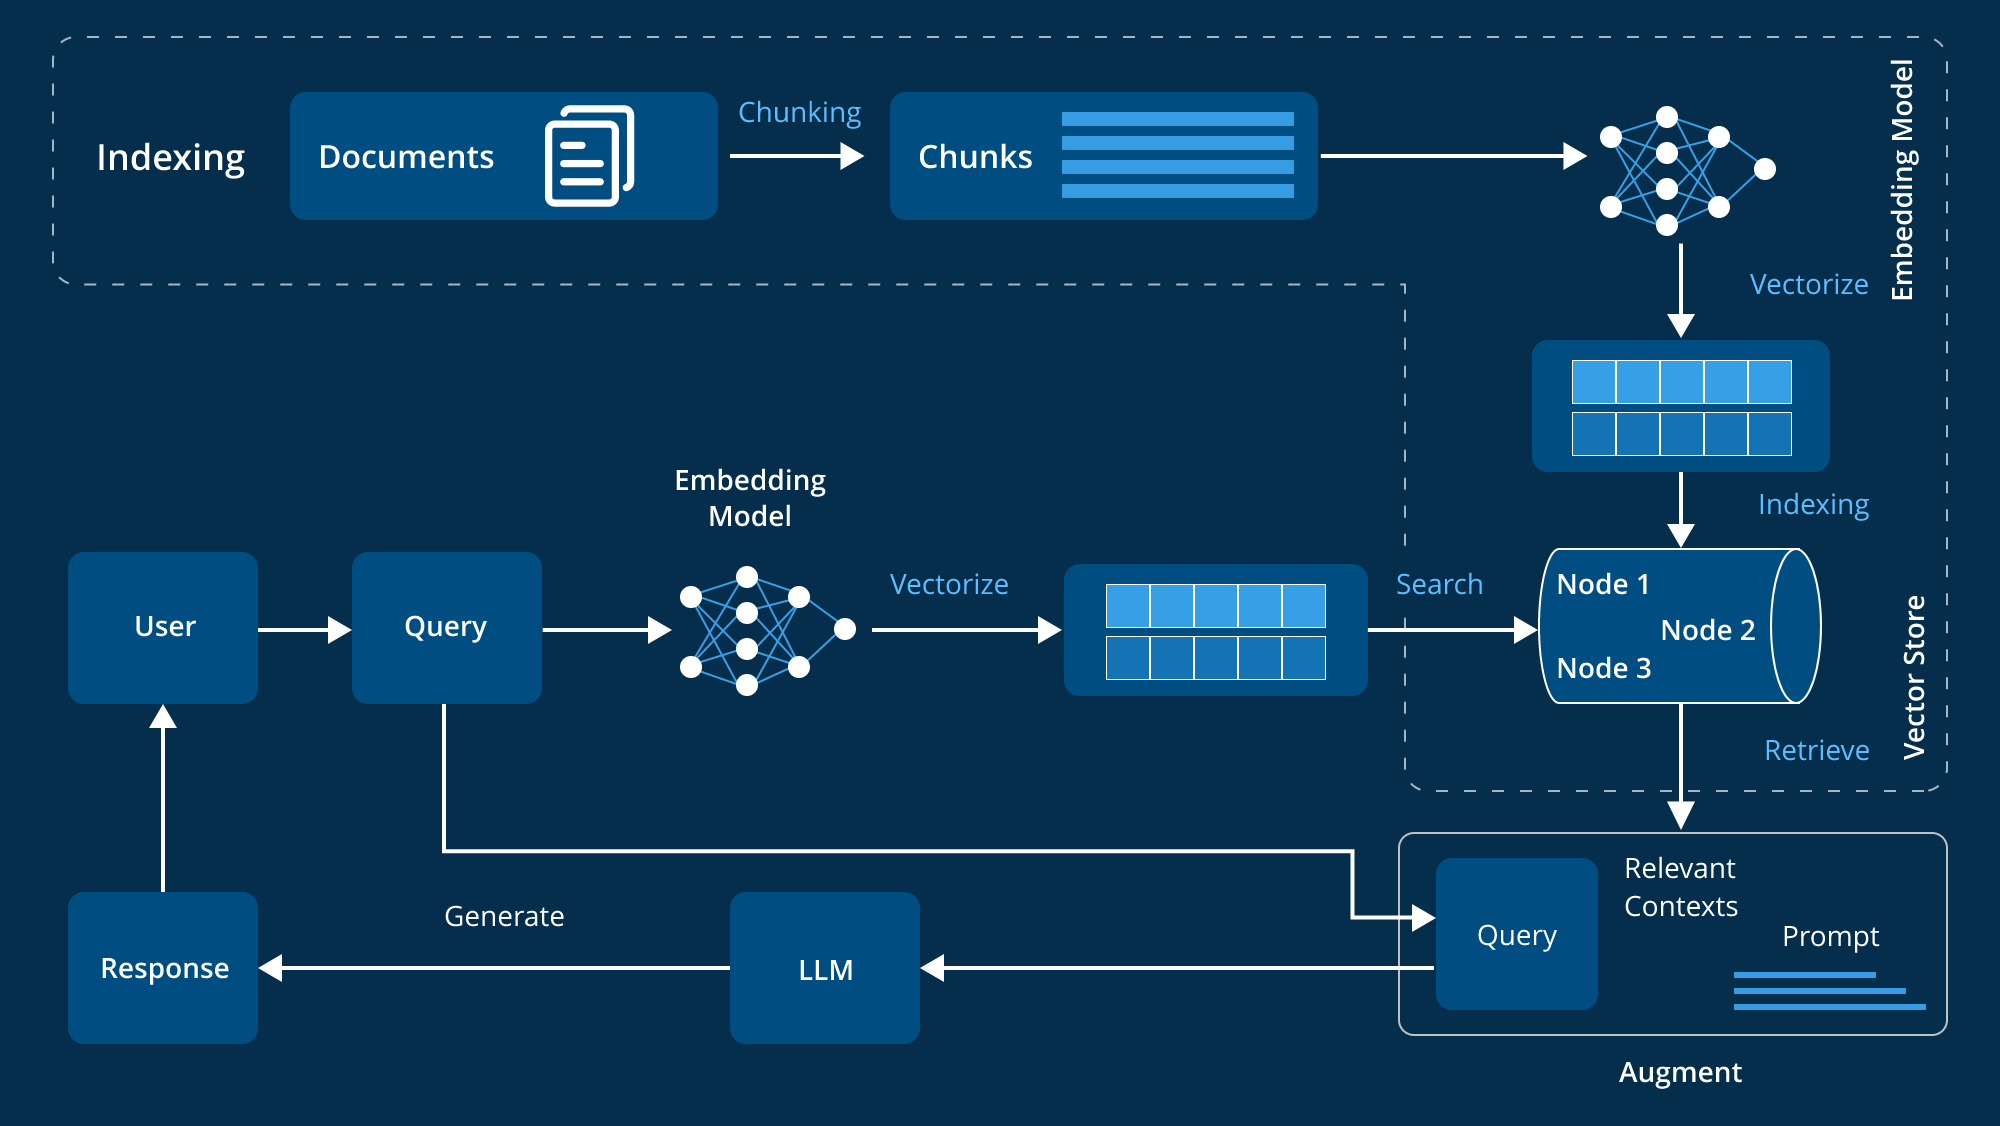
\includegraphics[width=0.9\textwidth]{images/chapter2/rag_architecture_2.png}
    \caption{High-level architecture of a Retrieval-Augmented Generation system.}
    \label{fig:rag_architecture}
\end{figure}

\section{Main Challenges}
The apparent simplicity of the Naive RAG pipeline conceals several intricate challenges that must be addressed to construct a robust and effective system \autocite{gao2024retrievalaugmented}.

\subsection{Ensuring Content Relevance}
The quality of the generated output is fundamentally dependent on the quality of the retrieved context. Should the retriever yield irrelevant or suboptimal documents, the LLM may disregard them or, more critically, integrate erroneous information into its response. A significant challenge is the \textit{lost in the middle problem}, wherein LLMs frequently fail to prioritize relevant information when it is interspersed with less pertinent segments within the context window \autocite{liu2023lost}. This phenomenon highlights the imperative for retrieval systems that not only identify relevant documents but also effectively rank them.

\subsection{Optimizing Retrieval vs. Generation Trade-offs}
An intrinsic trade-off exists between the velocity and comprehensiveness of the retrieval step. Retrieving a greater number of documents may enhance the probability of identifying accurate information, yet it concurrently augments the computational burden and the potential for noise introduction. The permissible length of the context provided to the LLM is constrained by its inherent context window size. As emphasized by Gao et al. (2024) \autocite{gao2024retrievalaugmented}, optimizing the selection of the most pertinent document chunks from the initial similarity search constitutes a significant challenge. Techniques like re-ranking retrieved results, which will be explored later in this thesis, are designed to address this trade-off.

\subsection{Handling Noisy or Conflicting Information}
Real-world data frequently exhibits characteristics of disorder and heterogeneity. The retrieved context may encompass contradictory facts or extraneous details. The RAG system must demonstrate resilience to such noise, and the LLM must possess the capacity to synthesize information from multiple sources, identify contradictions, and prioritize the most reliable data. Advanced RAG architectures, such as those employing query transformations or reranking, are designed to tackle this issue \autocite{gao2024retrievalaugmented, rag_fusion_2024}.

\subsection{Seamless Integration and Synthesis}
The LLM must be capable of seamlessly integrating the retrieved information into a coherent and linguistically natural response. This necessitates not merely the extraction of facts but also a comprehensive understanding of contextual nuances and their integration into a cohesive narrative that directly addresses the user's query. The fluency and relevance of the final output serve as direct indicators of the RAG system's efficacy.

\section{Vector Databases and Similarity Search}
The conceptualization of representing text as vectors within a multi-dimensional space for similarity comparison, foundational to modern vector databases, was initially advanced by the Vector Space Model (VSM) in 1975 \autocite{salton1975vector}. Vector databases are a cornerstone of modern RAG systems, serving as the indexed knowledge base. These databases operate by storing textual data as high-dimensional vectors, commonly referred to as \textit{embeddings}. Upon receipt of a query, it is similarly transformed into an embedding, and the database then identifies the vectors within its index that exhibit the highest proximity to the query vector.



\subsection{Measuring Similarity}
The predominant method for quantifying the distance between two vectors within the context of RAG is \textbf{cosine similarity}, which quantifies the cosine of the angle subtended by them. For two vectors, A and B, the cosine similarity is calculated as:
\begin{equation}
\text{Cosine Similarity} = \frac{A \cdot B}{\|A\| \|B\|}
\end{equation}
Where \(A \cdot B\) is the dot product of the two vectors, and \(\|A\|\) and \(\|B\|\) are their magnitudes. The result ranges from -1 (exactly opposite) to 1 (exactly the same).
Another common metric is \textbf{Euclidean distance}, which is the straight-line distance between two points in the vector space:
\begin{equation}
\text{Euclidean Distance} = \sqrt{\sum_{i=1}^{n} (A_i - B_i)^2}
\end{equation}

\subsection{The Advantage of Normalized Vectors}
For enhanced efficiency, it is standard practice to \textbf{normalize} the vectors prior to their storage in the database. A normalized vector has a magnitude (or L2 norm) of 1. The magnitude of a vector \(A = [a_1, a_2, \ldots, a_n]\) is computed as:

\begin{equation}
\|A\| = \sqrt{a_1^2 + a_2^2 + \cdots + a_n^2}
\end{equation}

When vectors undergo normalization, the denominator in the cosine similarity formula (\(\|A\| \|B\|\)) converges to 1. Consequently, the cosine similarity calculation simplifies to merely the \textbf{dot product} of the vectors, resulting in a substantially reduced computational cost:

\begin{equation}
\text{Cosine Similarity (normalized)} = A \cdot B
\end{equation}

This optimization obviates the computationally intensive square root operations required for calculating vector magnitudes, thereby enabling significantly accelerated similarity searches, a critical factor for real-time RAG applications.


\subsection{Indexing for Efficient Search}
To circumvent a brute-force search, vector databases employ specialized indexing algorithms for Approximate Nearest Neighbor (ANN) search. These algorithms, including Hierarchical Navigable Small World (HNSW) \autocite{hnsw_malkov_2018} and Inverted File (IVF) \autocite{ivf_zobel}, facilitate the efficient retrieval of the top-k most similar vectors without necessitating a comparison of the query vector to every individual vector in the database. This is paramount for attaining low-latency responses in large-scale RAG systems.

\section{Mitigating Hallucinations}
A primary advantage of RAG is its capacity to mitigate LLM hallucinations. By providing factual, verifiable context directly within the prompt, RAG anchors the model's response in empirical data. The LLM is instructed to formulate its answer based on the provided text, reducing its reliance on its internal, parametric knowledge, which may be outdated or incorrect.

However, RAG does not present a complete panacea. Hallucinations within RAG systems can predominantly originate from two sources: retrieval failure (e.g., the provision of irrelevant or inaccurate context) and generation deficiency (e.g., the LLM's misinterpretation or disregard of the provided context). Should the retrieved context be of suboptimal quality, contain subtle inaccuracies, or prove inherently misleading, the LLM may nonetheless produce a deficient response. Therefore, the quality of the retrieval process is paramount. A well-tuned retriever that provides accurate and relevant context is the first and most critical line of defense against hallucinations in a RAG system \autocite{gao2024retrievalaugmented}.